\documentclass[12pt,a4paper,titlepage,twoside,openright]{book}

% Use the UniMelb Dissertation Template
\usepackage{style/uomthesis}

% User defined commands
%%
%% VERSION HISTORY
%%    22 May 2006 - John Papandriopoulos - Original version
%%    12 Jul 2007 - John Papandriopoulos - Converted into template
%%    30 Sep 2015 - Maoyuan Liu - Draft version
%%

% -----
% Basic
% -----

\usepackage{fixltx2e}

% AMS packages
%\usepackage{amsfonts}
\usepackage{amssymb}
\usepackage{amsmath}
\usepackage{amsthm}
\usepackage[mathscr]{eucal}

\usepackage{color}
\usepackage{xcolor}

% Graphics
\usepackage{graphicx}
\usepackage{float}
%\usepackage{caption}

% For subfigures
%\usepackage{subfig}
%\usepackage{subfigure}


% --------------------
% Lists and references
% --------------------
\usepackage{url}
\usepackage[linktoc=all]{hyperref}
\hypersetup{
    colorlinks,
    citecolor=black,
    filecolor=black,
    linkcolor=black,
    urlcolor=black
}

% bibliography at the end of every chapter
\usepackage[numbers,sort&compress,sectionbib,square]{natbib}
\usepackage{chapterbib}

% List of index
\usepackage{makeidx}
\makeindex

% Glossary --> defitions of symbols and acronyms
\usepackage[toc,nonumberlist,nopostdot]{glossaries}
\makeglossaries
\setglossarystyle{treegroup}

% ------
% Layout
% ------

% Suppress "This page intentionally left blank."
\newcommand*\markblankpages{}

% set page margins
%   these margins are set by the A4 paper ratios, 1:sqrt(2)
%   paperheight/paperwidth = paperwidth/textwidth = paperheight/textheight = sqrt(2)
%   outer/inner = bottom/top = sqrt(2)
\usepackage[outer=36.02988mm,inner=25.47697mm,top=36.0317mm,bottom=50.9565mm]{geometry}
\newcommand*\symmetricmargin{
    \newgeometry{outer=30.7534mm,inner=30.7534mm,top=36.0317mm,bottom=50.9565mm}
}
\newcommand*\bookmargin{
    \newgeometry{outer=36.02988mm,inner=25.47697mm,top=36.0317mm,bottom=50.9565mm}
}

% we've already gone this far, why not go the whole mile
% set the text spacing 
\setstretch{1.414}

% For testing the formatting
\usepackage{lipsum}

% ---------
% Eye candy
% ---------
\usepackage[labelfont={bf,singlespacing},
            textfont={singlespacing},
            justification={justified,RaggedRight},
            singlelinecheck=false,
            margin=0pt,
            figurewithin=chapter,
            tablewithin=chapter]{caption}
\usepackage[titletoc]{appendix}

% fancy chapter titles and quotes at beginning of title
\usepackage[helvetica]{quotchap} 

% Draft watermark
\usepackage[contents={}]{background}
\usepackage[yyyymmdd,hhmmss]{datetime}
\newcommand*\DraftText{Draft compiled on \today\ at \currenttime}
\newcommand*\draft{
  \newcommand*{\archivalpapernote}{}
  \backgroundsetup{
    color=lightgray,
    position=current page.center,
    angle=90,
    vshift=0.45\paperwidth,
    opacity=1,
    scale=1,
    contents={\LARGE\ttfamily\DraftText}
  }
}

% --------------------------
% Macros and useful commands
% --------------------------

\newcommand*\cleartoleftpage{%
  \clearpage
  \ifodd\value{page}\hbox{}\newpage\fi
}


% set draft watermark
\draft

\begin{document}

    %%
    %% Front matter
    %%
    \begin{frontmatter}

        \frontmatterheadings

        % Dissertation title
\title{Working Title}

% Author
\author{Maoyuan Liu}

% Date of submission
\submissionmonth{January}
\submissionyear{2016}

% Department
\department{School of Chemistry}

% University
\university{\scshape The University of Melbourne}


        % the title page is centered horizontally
        \symmetricmargin
        \maketitle
        \bookmargin

        \begin{abstract}%

{\scshape A long time ago in a galaxy far far away...}

It is a period of civil war. Rebel spaceships, striking from a hidden base, have won their first victory against the evil Galactic Empire.

During the battle, rebel spies managed to steal secret plans to the Empire's ultimate weapon, the DEATH STAR, an armored space station with enough power to destroy an entire planet.

Pursued by the Empire's sinister agents, Princess Leia races home aboard her starship, custodian of the stolen plans that can save her people and restore freedom to the galaxy....

\end{abstract}

        \makedeclaration
        \begin{acknowledgements}
    I would like to thank Han Solo who ran the fastest parsec the likes of which the world has never seen the likes of which.
\end{acknowledgements}

        \begin{dedication}
	To my templator, John Papandriopoulos.
\end{dedication}


        {\singlespacing
            \tableofcontents

            \clearpage
            \addcontentsline{toc}{chapter}{List of Figures}
            \listoffigures

            \clearpage
            \addcontentsline{toc}{chapter}{List of Tables}
            \listoftables
        }

    \end{frontmatter}

    %%
    %% Main matter
    %%
    \begin{mainmatter}

        \mainmatterheadings

        % path to figures directory
\graphicspath{{figures/chapter-1/}}

%=========================================================================

\begin{savequote}[75mm]
Nulla facilisi. In vel sem. Morbi id urna in diam dignissim feugiat. Proin molestie tortor eu velit. Aliquam erat volutpat. Nullam    ultrices, diam tempus vulputate egestas, eros pede varius leo.
\qauthor{Quoteauthor Lastname}
\end{savequote}

\chapter{Introduction}
	\label{chapter:introduction}
	%

%=========================================================================

\section{Introduction}

\lipsum[1-6]\cite{Mao}
\index{a}
\myglossaryentry{lipsum}{lipsum}{Lorem Ipsum, a special type of fudge}{}
\myglossaryentry{dolor}{dolor}{No idea why}{parent={lipsum}}
\myglossaryentry{ibit}{ibit}{Sounds right, doesn't it?}{parent={lipsum}}
\myacronym{DFT}{density functional theory}
%\myglossaryentry{\ensuremath{\pi}}{pi}{Greek letter pi, \ensuremath{\Pi} does this work?}{symbol={\ensuremath{\pi}}, sort=pi}
\myglossaryentry{$\pi$}{pi}{Greek letter pi, \ensuremath{\Pi} does this work?}{symbol={$\pi$}}
\myacronym{RDF}{radial distribution function}
\myglossaryentry{radial distribution function}{radialdistributionfunction}{}{symbol={$g(r)$}}

\begin{figure}[h]
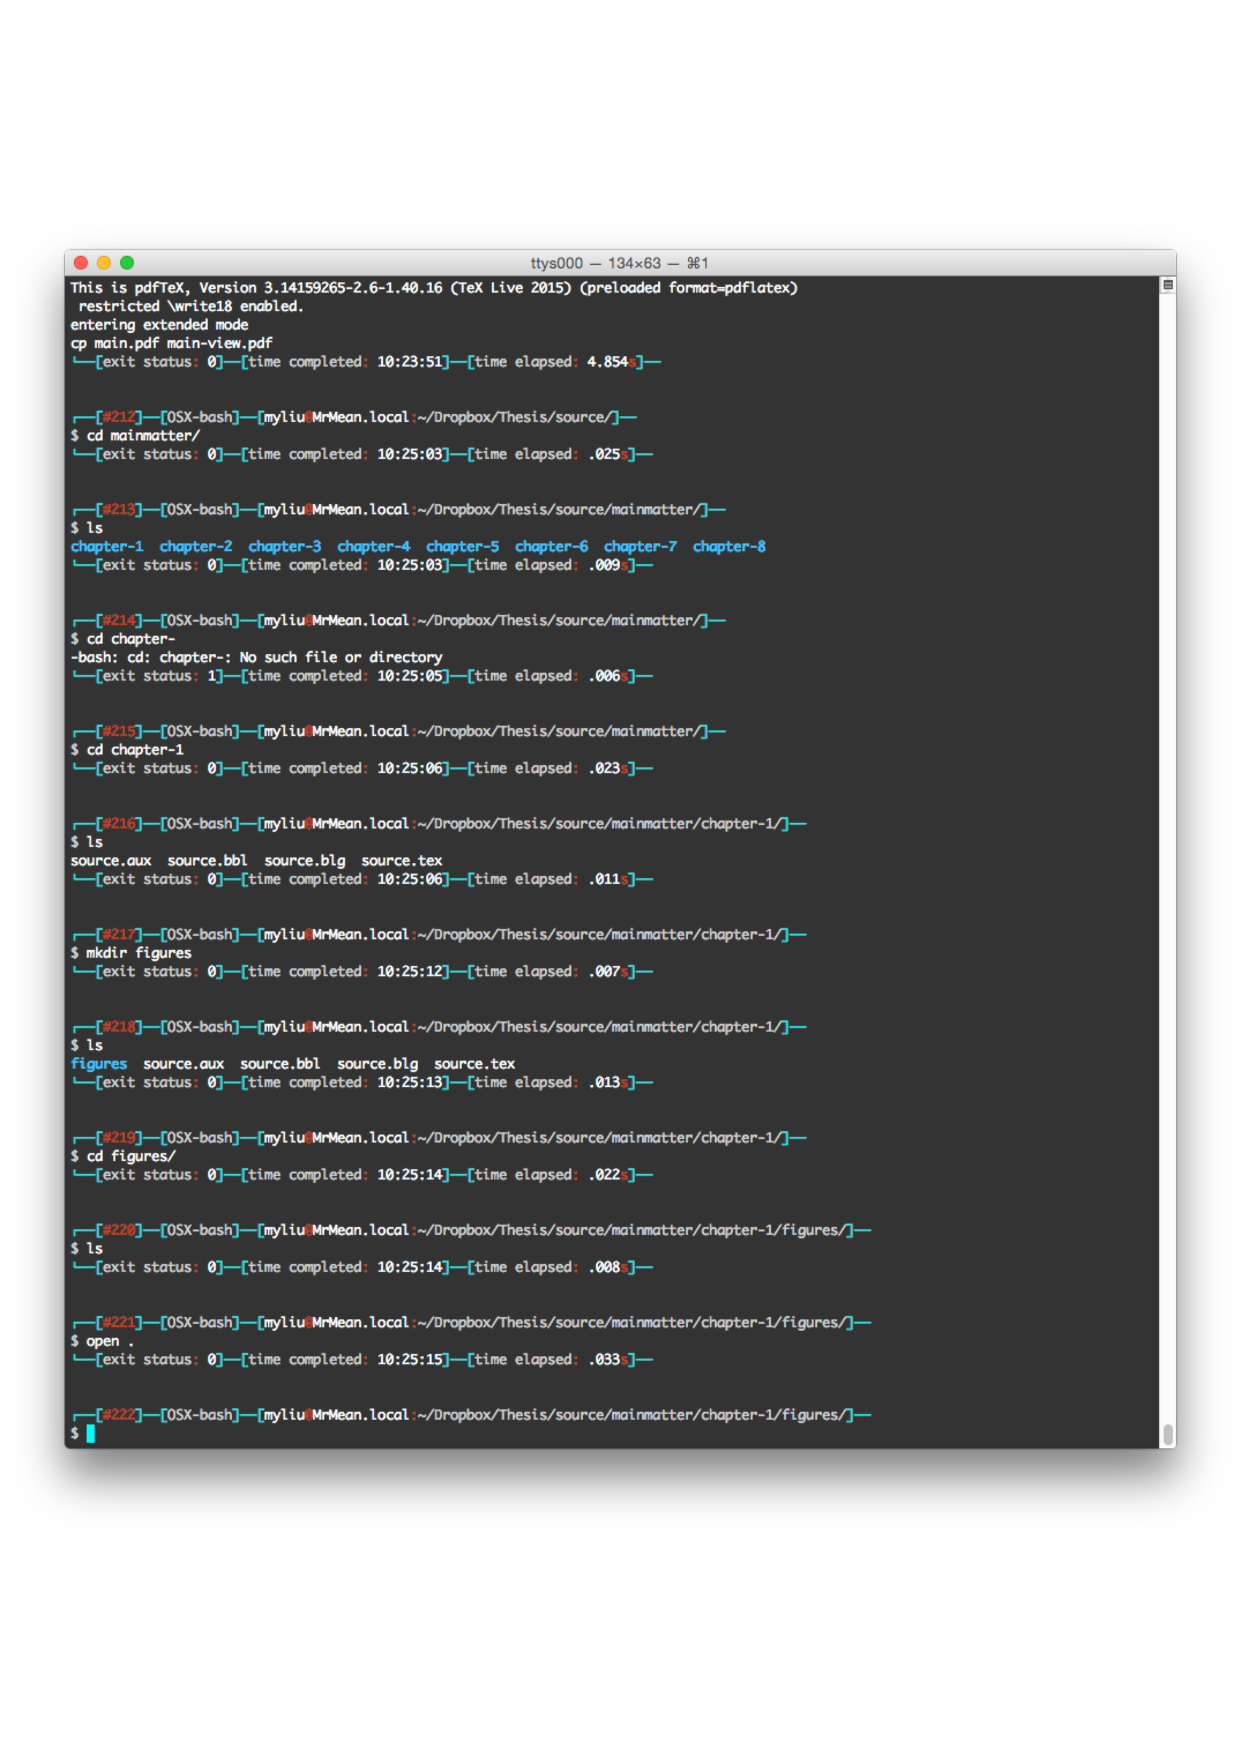
\includegraphics[height=0.7\textheight]{a.pdf}
\caption[This is a short caption]{This is a terminal screen for stuff.\cite{Mao}}
\end{figure}

%=========================================================================

\mybib{bib/test.bib}

        \chapter{The Phantom Menace}
	%\label{chapter:}

% preferred location for figures in this chapter
\graphicspath{{figures/chapter-2/}}

%=========================================================================

\begin{synopsis}
	In this chapter...
\end{synopsis}

%=========================================================================

\section{Introduction}

\lipsum[1-4] \index{amet}
\cite{Lorch1969}

\mybib{bib/test.bib}

        \chapter{The Empire Strikes Back}
	\label{chapter:empire-strikes-back}%
	%

% preferred location for figures in this chapter
\setfigurepath{figures/chapter-3}

%=========================================================================

\begin{synopsis}
	Synopsis.
\end{synopsis}

%=========================================================================

\section{Introduction}

\PARstart{U}{se} the force Luke...\cite{Salmon2006}

\mybib{bib/test.bib}

        % path to figures directory
\graphicspath{{figures/chapter-4/}}

%=========================================================================

\begin{savequote}[75mm]
Nulla facilisi. In vel sem. Morbi id urna in diam dignissim feugiat. Proin molestie tortor eu velit. Aliquam erat volutpat. Nullam    ultrices, diam tempus vulputate egestas, eros pede varius leo.
\qauthor{Quoteauthor Lastname}
\end{savequote}

\chapter{Return of the Sith}
  %\label{chapter:}

%=========================================================================

\section{Introduction}

\lipsum[15-19]
\cite{Salmon2006}

%=========================================================================

\mybib{bib/test.bib}

        \chapter{The Phantom Menace}
	\label{chapter:phantom-menace}%
	%

% preferred location for figures in this chapter
\setfigurepath{figures/chapter-5}

%=========================================================================

\begin{synopsis}
	Synopsis.
\end{synopsis}

%=========================================================================

\section{Introduction}

\PARstart{U}{se} the force Luke...


        % path to figures directory
\graphicspath{{figures/chapter-6/}}

%=========================================================================

\begin{savequote}[75mm]
Nulla facilisi. In vel sem. Morbi id urna in diam dignissim feugiat. Proin molestie tortor eu velit. Aliquam erat volutpat. Nullam    ultrices, diam tempus vulputate egestas, eros pede varius leo.
\qauthor{Quoteauthor Lastname}
\end{savequote}

\chapter{The Empire Strikes Back}
  %\label{chapter:}

%=========================================================================

\section{Introduction}

\lipsum[100]
\cite{Salmon2006}

%=========================================================================

\mybib{bib/test.bib}

        \chapter{Return of the Jedi}
	%\label{chapter:empire-strikes-back}%

% preferred location for figures in this chapter
\graphicspath{{figures/chapter-7/}}

%=========================================================================

\begin{synopsis}
	Synopsis.
\end{synopsis}

%=========================================================================

\section{Introduction}

\lipsum[10]

\mybib{bib/test.bib}


    \end{mainmatter}

    %%
    %% Appendix
    %%
    \begin{appendices}

        % path to figures directory
\graphicspath{{figures/appendix/}}

%=========================================================================

\begin{savequote}[75mm]
Nulla facilisi. In vel sem. Morbi id urna in diam dignissim feugiat. Proin molestie tortor eu velit. Aliquam erat volutpat. Nullam    ultrices, diam tempus vulputate egestas, eros pede varius leo.
\qauthor{Quoteauthor Lastname}
\end{savequote}

\chapter{The Force Awakens}
		\label{appendix-1}

%=========================================================================

\section{Introduction}

\lipsum[50-55]\cite{Lucas7}

%=========================================================================

\mybib{bib/test.bib}


        % path to figures directory
\graphicspath{{figures/appendix/}}

%=========================================================================

\begin{savequote}[75mm]
Nulla facilisi. In vel sem. Morbi id urna in diam dignissim feugiat. Proin molestie tortor eu velit. Aliquam erat volutpat. Nullam    ultrices, diam tempus vulputate egestas, eros pede varius leo.
\qauthor{Quoteauthor Lastname}
\end{savequote}

\chapter{Episode VIII}
		\label{appendix-2}

%=========================================================================

\section{Not named yet}

\lipsum[56-70]\cite{Lucas8}

%=========================================================================

\mybib{bib/test.bib}



    \end{appendices}

    %%
    %% Back matter
    %%
    \glsaddall
    \begin{backmatter}
        \frontmatterheadings

        \printglossary[title=Definition of Symbols and Acronyms]

        \clearpage
        \addcontentsline{toc}{chapter}{Index}
        \printindex

        
\cleartoleftpage
\par\vbox{}\null\vfill\nopagebreak
%\vspace*{350pt}

%\begin{center}
%\footnotesize
\small
\noindent
\parbox{105mm}{\textsc{This thesis was typeset} using \LaTeX. The template used by this thesis was adapted from templates by John \mbox{Papandriopoulos} (\url{http://jpap.org/projects.html}) and Jordan Suchow (\url{https://github.com/suchow/Dissertate}). A template that can be used to format a PhD dissertation with this look \textit{\&} feel has been released under \href{http://creativecommons.org/licenses/by-nc-nd/3.0/}{\textsc{cc by-nc-nd 3.0}} license, and can be found online at \href{https://github.com/XXXX} or from its lead author, Maoyuan Liu, at \mbox{\href{mailto:contact@mao.id.au}{contact@mao.id.au}}.}
%\end{center}


    \end{backmatter}

\end{document}
